\documentclass[final,nocolorBG,a4,mobius,nototal,pdf,slideColor]{prosper}

\addtolength{\textheight}{-1cm}
\usepackage[T1]{fontenc}
\usepackage[latin1]{inputenc}
\pagestyle{plain}
\usepackage{amsmath}
\usepackage{graphicx}
\usepackage{amssymb}
\usepackage{alltt}
\usepackage{xspace}
\makeatletter

\newcommand{\textttbf}[1]{\texttt{\textbf{#1}}}

\input{colour.tex}
\newcommand{\varHook}[1]{\mbox{\slshape #1}}
\newcommand{\codeHook}[1]{\mbox{\ttfamily #1}}

\def \bsl       {\symbol{92}}
\def \unsc      {\symbol{95}}

\usepackage{pstricks,pst-node,pst-text,pst-3d}
\usepackage{epsfig}

%\usepackage{colordvi}
\usepackage{epsf}

\input{prooftree} 

\usepackage{colours}

\title{\vspace*{-1em}\Blue{Bytecode Modeling Language}\bigskip\\
}
\subtitle{}
\author{  \Blue{Marieke Huisman}\\
  INRIA Sophia Antipolis}
\institution{\ \\ \ \\ \ \\ \ \\ \ \\ \ \\

\includegraphics[width=2.5cm]{mobius_transparent.ps}\hspace*{5cm}
\includegraphics[width=2.5cm]{logo_inria.ps}}

\slideCaption{BML}



\begin{document}

\maketitle

\begin{slide}{Why do you need to specify your executable code?}
\begin{itemize}
\item Executable code not accompanied by (specified) source
\item Untrusted compiler
\item Application developed directly at bytecode level
\end{itemize}
\end{slide}

\begin{slide}{Proof carrying code scenario}
\vspace*{-1em}
\begin{center}
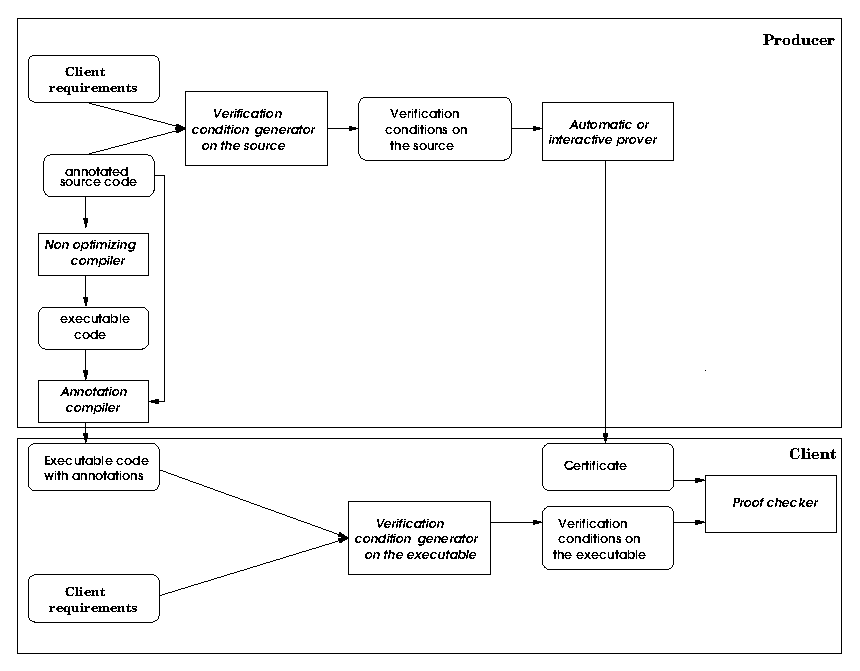
\includegraphics[height=.9\textheight]{PPO.eps}
\end{center}
\end{slide}

\begin{slide}{Bytecode Modeling Language (BML)}
\begin{itemize}
\item Bytecode cousin of Java Modeling Language (JML)
\item Format to store specifications in class file
\item Compiler for JML specifications defined
\end{itemize}
\end{slide}

\begin{slide}{Syntax for BML predicates}
\begin{tabular}{lll}
\multicolumn{2}{l}{\varHook{predicate} ::= \(\ldots\)}\smallskip\\
\multicolumn{2}{l}{\varHook{unary-expr-not-plus-minus} ::= \(\ldots\)}\\
\hspace*{1cm} & \(\mid\) \varHook{primary-expr} [\varHook{primary-suffix}]\(\ldots\)\\ 

\multicolumn{3}{l}{\varHook{primary-suffix} ::= \codeHook{.} \varHook{ident}
\(\mid\) \codeHook{(} [\varHook{expression-list}] \codeHook{)}}\\
& \(\mid\) \codeHook{[} \varHook{expression} \codeHook{]}\\

\multicolumn{2}{l}{\varHook{primary-expr} ::= 
\Blue{\codeHook{\#}\varHook{natural}}} \\
&\(\mid\) \Blue{\codeHook{lv[}\varHook{natural}\codeHook{]}} \\
&\(\mid\) \Blue{\varHook{bml-primary}}\\
&
\multicolumn{2}{l}{\(\mid\) \varHook{constant} \(\mid\)
\codeHook{super}
\(\mid\) \codeHook{true} \(\mid\) \codeHook{false} \(\mid\)
\codeHook{this}} \\
& \(\mid\) \codeHook{null} 
\(\mid\) \codeHook{(}\varHook{expression}\codeHook{)}
\(\mid\) \varHook{jml-primary}\\
\end{tabular}
\end{slide}

\begin{slide}{Syntax for BML predicates (2)}
\begin{tabular}{lll}

\multicolumn{2}{l}{\varHook{bml-primary} ::= \Blue{\codeHook{cntr}}} \\
&\(\mid\) \Blue{\codeHook{st(}\varHook{additive-expr}\codeHook{)}} \\
&\(\mid\) \Blue{\codeHook{length(}\varHook{expression}\codeHook{)}} 
\end{tabular}

\end{slide}

\begin{slide}{BML specifications}
\begin{itemize}
\item Class and method specifications as in JML
\item Loop specifications
\item Assert and other annotation statements
\item All BML specifications respect structural and typing constraints \`a la BCV
\end{itemize}
\end{slide}

\begin{slide}{Example}
\begin{alltt}
\{| \Blue{requires lv[1] > 0}
   \Blue{ensures lv[0].\#24 <= \bsl\(\strut\)old(lv[0].\#24) + 
                 lv[1] * (lv[1] + 1) / 2 |\}}
 0 iconst_1

16 putfield \#24 <Bill.sum>
19 iinc 2 by 1
\Blue{loop_inv 0 <= lv[2] && 0 <= lv[0].\#24 && 
         lv[2] <= lv[1] + 1 && 
         lv[0].\#24 <= \bsl\(\strut\)old(lv[0].\#24) 
               + (lv[2] - 1) * lv[2]/2}
22 iload_2 // entry loop

31 ireturn
\end{alltt}

\end{slide}

\begin{slide}{Storing BML specifications in the class file}
\begin{itemize}
\item User specific attributes
\item Does not affect execution of JVM
\item Ingredients
\begin{itemize}
\item a second constant pool
\item ghost fields attribute
\item model fields attribute
\item class invariants attribute (both static and object)
\item constraints  attribute (both static and object)
\end{itemize}
\end{itemize}
\end{slide}

\begin{slide}{Attribute for ghost fields}
\begin{tabular}[t]{l}
Ghost\unsc Field\unsc attribute \{\\
\hspace*{1em}
\begin{tabular}{l}
u2  attribute\unsc name\unsc index; \\
u4  attribute\unsc length;\\
u2  fields\unsc count;\\
\{\begin{tabular}[t]{l} 
    u2 access\unsc flags; \\  
    u2 name\unsc index;\\
    u2 descriptor\unsc index;\\
  \end{tabular}\\
\} fields[fields\unsc count]; \} \\
\end{tabular}
\end{tabular}
\end{slide}

\begin{slide}{JML to BML compiler}
\begin{itemize}
\item Compilation of ghost and model field declarations

\item Linking and resolving of source data structures

\item Locating instructions for annotation statements

\item Compilation of JML predicates

\item Generation of user-specific class attributes
\end{itemize}
\end{slide}

\begin{slide}{Current work}
\begin{itemize}
\item BML Reference Manual
\item Settling many small details
\item Current issues:
\begin{itemize}
\item Which part of JML to cover
\item Desugaring of specifications
\item Evaluation order for statement annotations
\end{itemize}
\end{itemize}
\end{slide}

\begin{slide}{A few words about verification}
\begin{itemize}
\item Direct verification condition generator vs. translation into guarded commands 
\item Preservation of proof obligations
\end{itemize}
\end{slide}

\begin{slide}{Mobius tool set}
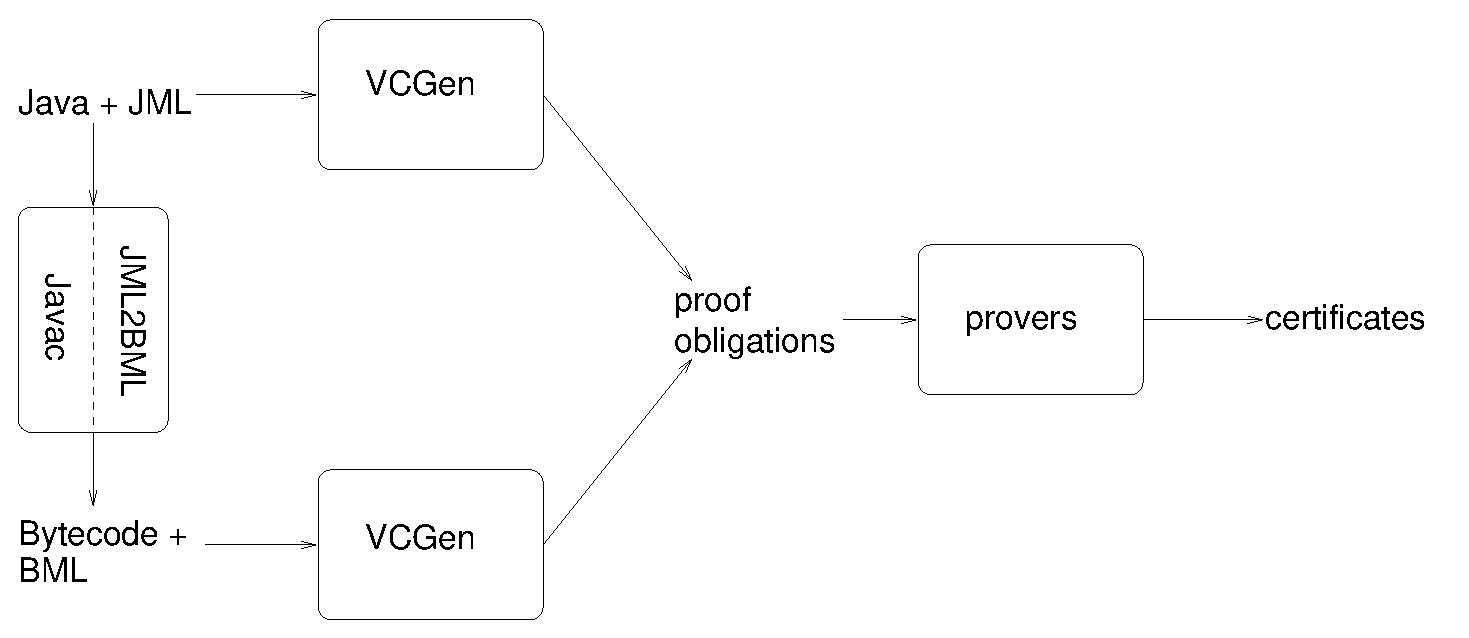
\includegraphics[width=\textwidth]{toolset.eps}

\end{slide}

\begin{slide}{Related work}
\begin{itemize}
\item Logics to reason about bytecode [Bannwart \& M\"uller (Bytecode 2005), MRG project (TPHols 2004)]
\item JVer verifies bytecode annotated with source code level specifications
[Chander \emph{et al.} (CAV 2005)]
\item Boogie project [Barnett \emph{et al.}]
\item Assert in Java 1.5
\item Extended Virtual Platform: compile JML annotations for run-time checking
[Alagic \emph{et al.}]
\end{itemize}
\end{slide}

\begin{slide}{Highlights of BML}
\begin{itemize}
\item Bytecode cousin of Java Modeling Language (JML)
\item Easy reading of specifications
\item Specifications stored together with the class file
\item Compiler for JML specifications defined
\end{itemize}
\end{slide}

\begin{slide}{To know more about the details...}
\begin{itemize}
\item Paper presented at FASE 2007
\item The webpage with the BML Reference Manual (under development)
\begin{center}
\texttt{http://www-sop.inria.fr/everest/BML}
\end{center}
\end{itemize}
\end{slide}

\end{document}
